% Author: Seongjin Lee
% Hanyang University, Seoul, Korea
% esos.hanyang.ac.kr
% 2016-09-20
% note: some slides are adopted from  \url{www.cs.stevens.edu/~jschauma/631A/}
% https://github.com/resourceful/lecture_sysprog/

\documentclass[newPxFont,sthlmFooter,nooffset]{beamer}
\usepackage{kotex}
%\usetheme{sthlm}
\usepackage{../beamer_template/beamerthemesthlm}
\hypersetup{pdfauthor={Seongjin Lee (insight@gnu.ac.kr)},
            pdfsubject={Lecture Note: System Programming},
            pdfkeywords={Lecture Note, System Programming, class, (under)graduate},
            pdfmoddate={D: \pdfdate},
            pdfcreator={Seongjin Lee}
            pdfpresentor={Gyuri Chang}}

%\setbeamertemplate{footline}[text line]{%
%    \parbox{\linewidth}{\vspace*{-8pt} \insertsectionhead  \hfill\insertshortauthor\hfill\insertpagenumber}}
%\setbeamertemplate{navigation symbols}{}




\title{System Programming}
\subtitle{Topic 4: System Data Files and Process Environment}
\author[SJL]{Seongjin Lee}
\institute{\href{mailto:insight@gnu.ac.kr}{insight@gnu.ac.kr}\\\url{http://open.gnu.ac.kr}\\Systems Research Lab.\\Gyeongsang National University\\Presentor: Gyuri Chang}
\date{\today}

\begin{document}



\frame[plain]{\titlepage}

\frame{\frametitle{Table of contents}\tableofcontents}


%---------------------------------------------------------

\section{Password, Group, and other system files}

\begin{frame}[t]
  \frametitle{introduction}
A \textsc{Unix} system requires numerous data files for normal operations
\begin{itemize}
\item \texttt{/etc/passwd} - for user log-in or \texttt{ls -l}, etc
\item \texttt{/etc/group} - for group information
\end{itemize}

These data files have been ASCII text files and were read with the standard I/O libaray.

\begin{itemize}
\item sequential scan of such files became time consuming for a large system
\end{itemize}


We want to other data format other than ASCII, but still provide an interface for any application.

\end{frame}




\subsection{Password files}








\begin{frame}[containsverbatim,t]
  \frametitle{Password File}

The UNIX System’s password file \texttt{<pwd.h>}, called the user database by POSIX.1, contains the following fields

\begin{figure}[h]
  \centering
  \includegraphics[width=\textwidth]{figure/fig6-1_etc_passwd.png}
  \caption{Fileds in \texttt{/etc/passwd} file}
\end{figure}
\vspace{-1em}

On your machine, you can see the contents by typing \texttt{cat /etc/passwd}
\lstinputlisting[aboveskip=0em,lineskip=0em]{codes/sample_passwd}

\end{frame}




\begin{frame}[t]
  \frametitle{Password File cnt'd}
  \begin{itemize}
  \item if ecrypted passwd field is empty, it usually means that the user does not have passwd
  \item shell field contains the name of a program to be used as the login shell for the user. If this field is empty, the default is \texttt{/bin/sh}
  \item \texttt{/dev/null}, \texttt{/bin/false}, or \texttt{/bin/true} in the shell field prevents a particular user from logging in to a system
  \item \texttt{nobody} user name can be used to allow people to log, but with a user ID (65534) and group ID (65534)
  \end{itemize}
\end{frame}

\begin{frame}[containsverbatim,t]
  \frametitle{Password File API }
\begin{codedef}
#include <pwd.h>
struct passwd *getpwuid(uid_t uid);
struct passwd *getpwnam(const char *name);
// Both return: pointer if OK, NULL on error
\end{codedef}

\texttt{getpwuid} function is used by \texttt{ls(1)} program to map the numberical user ID contained in an i-node into a user's login name

\texttt{getpwnam} function is used by the \texttt{login(1)} program when we enter our login name

Both functions return a pointer to \texttt{passwd} structure that the functions fill in

They are only for looking up either a login name or a user ID
\end{frame}




\subsection{Group files}

\begin{frame}[t]
  \frametitle{Group File}
The UNIX System’s group file, called the group database by POSIX.1, contains the fields shown in the figure. These fields are contained in a group structure that is defined in \texttt{<grp.h>}.



\begin{figure}[h]
  \centering
  \includegraphics[width=\textwidth]{figure/fig6-4_group.png}
  \caption{Fields in \texttt{/etc/group} file}
\end{figure}

The field \texttt{gr\_mem} is an array of pointers to the user names that belong to this group. This array is terminated by a null pointer.

\end{frame}



\begin{frame}[containsverbatim,t]
  \frametitle{Group File API}

We can look up either a group name or a numerical group ID with the following

\begin{codedef}
#include <grp.h>
struct group *getgrgid(gid_t gid);
struct group *getgrnam(const char *name);
// Both return: pointer if OK, NULL on error
\end{codedef}

Like the password file functions, both of these functions normally return pointers to a static variable, which is overwritten on each call.

Followings are used for searching the entire group file
\begin{codedef}
#include <grp.h>
struct group *getgrent(void);  // returns next group entry in file each time it's called, but not in order
// Returns: pointer if OK, NULL on error or end of file
void setgrent(void);  // rewinds to the beginning of entries
void endgrent(void);  // closes the file
\end{codedef}


\end{frame}



\subsection{Others System Databases Files}

\begin{frame}[t]
  \frametitle{Other System Database Files}
There are other system files and has similar routines for accessing them


\begin{figure}[h]
  \centering
  \includegraphics[width=\textwidth]{figure/fig6-6_similar.png}
  \caption{Similar routines for accessing system data files}
\end{figure}


\begin{itemize}
\item \textbf{\texttt{get}} function reads the next record, opening the file if necessary
\item \textbf{\texttt{set}} function that opens the file, if not already open, and rewinds the file
\item \textbf{\texttt{end}} entry that closes the data file. We always have to call this function when we're done.
\end{itemize}

\end{frame}


\begin{frame}[containsverbatim,t]
  \frametitle{System Identification}
POSIX.1 defines the uname function to return information on the current host and operating system

\begin{codedef}
#include <sys/utsname.h>
int uname(struct utsname *name);
// Returns: non-negative value if OK, −1 on error
\end{codedef}

{\footnotesize
  \begin{itemize}
  \item We pass the address of a \texttt{utsname} structure to this function, and the function then fills it in.
  \item The structure contains fields like sysname, nodename, release, version, and machine; but, they depend on the implementation
  \item This is used by the shell command \texttt{uname(1)}
  \end{itemize}
}


\begin{codedef}
#include <unistd.h>
int gethostname(char *name, int namelen);
// Returns: 0 if OK, −1 on error
\end{codedef}
Historically, BSD-derived systems provided the gethostname function to return only the name of the host


\end{frame}


\subsection{Time and Date}

\begin{frame}[t]
  \frametitle{Time and Date Routines}
The basic time service provided by the \textsc{Unix} kernel counts the number of seconds that have passed since the Epoch: 00:00:00 January 1, 1970, Coordinated Universal Time (UTC).
\begin{itemize}
\item they are represented in a \texttt{time\_t} data type
\item they are called \textit{calendar times} and represent both the time and the date
\end{itemize}



The \textsc{Unix} System has always differed from other operating systems in
\begin{itemize}
\item keeping time in UTC instead of the local time
\item automatically handling conversions, such as daylight saving time,
\item keeping the time and date as a single quantity.
\end{itemize}


\end{frame}

\begin{frame}[containsverbatim,t]
  \frametitle{Time and Date Routines API}
The \texttt{time} function returns the current time and date
\begin{codedef}
#include <time.h>
time_t time(time_t *calptr);
// Returns: value of time if OK, −1 on error
\end{codedef}
\begin{itemize}
\item The time value is always returned as the value of the
  function.
\item If the argument is non- null, the time value is also
  stored at the location pointed to by \textit{calptr}
\end{itemize}
\end{frame}


\begin{frame}[containsverbatim,t]
  \frametitle{Time and Date Routines cnt'd}

The \texttt{clock\_gettime} function can be used to get the time of the specified clock

\begin{codedef}
#include <sys/time.h>
int clock_gettime(clockid_t clock_id, struct timespec *tsp); // get the time
int clock_getres(clockid_t clock_id, struct timespec *tsp); // resolution of a system clock
int clock_settime(clockid_t clock_id, const struct timespec *tsp); // set the time
// Returns: 0 if OK, −1 on error
\end{codedef}

\begin{figure}[h]
  \centering
  \includegraphics[width=\textwidth]{figure/fig6-8_clock.png}
  \caption{Clock type identifiers}
\end{figure}

\end{frame}

\begin{frame}[containsverbatim,t]
  \frametitle{Time and Date Routines cnt'd}
This function is now obsolete. However, a lot of programs stil use it, because it provides greater resolution (up to a microsecond) than the \texttt{time} function
\begin{codedef}
int gettimeofday(struct timeval *restrict tp, void *restrict tzp);
// Returns: 0 always
\end{codedef}


\end{frame}


\begin{frame}[containsverbatim,t]
  \frametitle{Time and Date Routines cnt'd: formating}

\begin{codedef}
#include <time.h>
size_t strftime(char *restrict buf, size_t maxsize, const char *restrict format, const struct tm *restrict tmptr);
size_t strftime_l(char *restrict buf, size_t maxsize, const char *restrict format, const struct tm *restrict tmptr, locale_t locale);
// Both return: number of characters stored in array if room, 0 otherwise
\end{codedef}

The strftime and \texttt{strftime\_l} functions are the same, except that the \texttt{strftime\_l} function allows the caller to specify the locale as an argument.

\end{frame}






\begin{frame}[containsverbatim,t]
  \frametitle{Time and Date Routines cnt'd: tm structure}

\begin{codedef}
struct tm {         /* a broken-down time */
     int  tm_sec;   /* seconds after the minute: [0 - 60] */
     int  tm_min;   /* minutes after the hour: [0 - 59] */
     int  tm_hour;  /* hours after midnight: [0 - 23] */
     int  tm_mday;  /* day of the month: [1 - 31] */
     int  tm_mon;   /* months since January: [0 - 11] */
     int  tm_year;  /* years since 1900 */
     int  tm_wday;  /* days since Sunday: [0 - 6] */
     int  tm_yday;  /* days since January 1: [0 - 365] */
     int  tm_isdst; /* daylight saving time flag: <0, 0, >0 */
};
\end{codedef}


\end{frame}





\subsection{Last Words}



\begin{frame}[containsverbatim,t]
  \frametitle{How to create a patch file}
\begin{columns}[t]
\begin{column}{0.45\textwidth}
The original file \texttt{foo.c}
\begin{lstlisting}
#include <stdio.h>

int main() {
printf("Hello World\n");
}
\end{lstlisting}
\end{column}
\begin{column}{0.45\textwidth}
Your modified file \texttt{foobar.c}
\begin{lstlisting}
#include <stdio.h>

int main(int argc, char *argv[]) {
printf("Hello World\n");
return 0;
}
\end{lstlisting}
\end{column}
\end{columns}

Create the patch file using diff command \\ \texttt{diff -u foo.c foobar.c > foobar.patch }

{\footnotesize
\lstinputlisting[xleftmargin=15em,lineskip=0em]{codes/foobar.patch}
}
\end{frame}


\section{Process Environment}

\begin{frame}[t]
  \frametitle{Introduction}
In this chapter, we'll see
\begin{itemize}
\item how the \texttt{main} function is called when the program is executed
\item called when the program is executed
\item how command-line arguments are passed to the new program
\item what the typical memory layout looks like
\item how to allocate additional memory
\item how the process can use environment variables
\item and various ways for the process to terminate
\item the \texttt{longjmp} and \texttt{setjmp} functions and their interaction with the stack
\end{itemize}
We finish the chapter by examining the resource limits of a process.
\end{frame}



\subsection{Process Creation and Termination }

\begin{frame}[containsverbatim,t]
  \frametitle{\texttt{main} Function}
\begin{codedef}
int main(int argc, char *argv[]);
\end{codedef}
\begin{itemize}
\item \textit{argc}: the number of commands-line arguments
\item \textit{argv}: an array of pointers to the arguments
\end{itemize}

The executable program file specifies this routine as the starting address for the program;
\begin{itemize}
\item this is set up by the link editor when it is invoked by the C
  compiler.
\item This start-up routine takes values from the kernel---the
  command-line arguments and the environment---and sets things up
\end{itemize}

\end{frame}



\begin{frame}[t]
  \frametitle{Process Termination}

There are eight ways for a process to terminate

Normal termination
\begin{itemize}
\item Return from \texttt{main}
\item Calling \texttt{exit}
\item Calling \texttt{\_exit} or \texttt{\_Exit}
\item Return of the last thread from its start routine
\item Calling \texttt{pthread\_exit} from the last thread
\end{itemize}

Abnormal termination (We'll discuss them later)
\begin{itemize}
\item calling \texttt{abort}
\item Receipt of a signal
\item Response of the last thread to a cancellation request
\end{itemize}

\end{frame}

\begin{frame}[containsverbatim,t]
  \frametitle{exit(3) Functions}
Following functions terminate a program normally
\begin{codedef}
#include <stdlib.h>
void exit(int status); // return to the kernel after some cleanup
void _Exit(int status); // return to the kernel immediately

#include <unistd.h>
void _exit(int status);  // return to the kernel immediately
\end{codedef}

\end{frame}

\begin{frame}[t]
  \frametitle{exit(3) Functions}
All three exit functions expect a single integer argument, which we
call the exit status. E.g., \texttt{exit(0);}

Most UNIX System shells provide a way to examine the exit status of a
process.

The exit status of the process is undefined, if
\begin{itemize}
\item any of these functions is called without an exit status,
\item main does a return without a return value, or
\item the main function is not declared to return an integer,
\end{itemize}

\end{frame}


\begin{frame}[containsverbatim,t]
  \frametitle{atexit(3) function}
With ISO C, a process can register at least 32 functions that are automatically called by
\texttt{exit}. These are called \textit{exit handlers} and are registered by calling the \texttt{atexit} function.

\begin{codedef}
#include <stdlib.h>
int atexit(void (*func)(void));
// Returns: 0 if OK, nonzero on error
\end{codedef}


\end{frame}





\subsection{Environments}

\begin{frame}
  \frametitle{Command-Line Arguments}
When a program is executed, the process that does the exec can pass command-line arguments to the new program.

\texttt{cd codes; make echoall}

\lstinputlisting[lineskip=-5pt]{codes/echoall.c}

try,
\texttt{./echoall arguments tests}

This you might want to test
\begin{itemize}
\item How many arguments can you pass
\item how can you insert multiple lines of text as arguments
\end{itemize}
\end{frame}

\begin{frame}[t]
  \frametitle{Environment List}
Each program is also passed an environment list
\begin{itemize}
\item it is an array of character pointers
\item each pointer containing the address of a null-terminated C
  string
\item The address of the array of pointers is contained in the global variable environ \texttt{extern char **environ;}
\end{itemize}

\begin{figure}[h]
  \centering
  \includegraphics[width=0.7\textwidth]{figure/fig7-5_environment.png}
  \caption{Environment consisting of five C character strings}
\end{figure}
\end{frame}

\begin{frame}[t]
  \frametitle{Environment Variables}
\begin{figure}[h]
  \centering
  \includegraphics[width=0.9\textwidth]{figure/fig7-7_environment.png}
  \caption{Environment consisting of five C character strings}
\end{figure}
\end{frame}

\begin{frame}[t]
  \frametitle{Environment List cnt'd}
ISO C specifies that the main function be written with two arguments

POSIX.1 specifies that environ should be used instead of the (possible) third argument
\begin{itemize}
\item Access to specific environment variables is normally through the
  \texttt{getenv} and \texttt{putenv} functions
\item But to go through the entire environment, the environ pointer must be used
\end{itemize}

\end{frame}



\begin{frame}[containsverbatim,t]
  \frametitle{Environment List APIs}

\begin{codedef}
#include <stdlib.h>
char *getenv(const char *name);
// Returns: pointer to value associated with name, NULL if not found
int putenv(char *str);
// Returns: 0 if OK, nonzero on error
int setenv(const char *name, const char *value, int rewrite);
int unsetenv(const char *name);
// Both return: 0 if OK, −1 on error
\end{codedef}
{\footnotesize
\begin{table}[h]
  \centering
  \begin{tabular}{l | c c | *{4}{c}  }
    Fuction & ISO C & POSIX.1 & \parbox{5em}{\centering FreeBSD 8.0} & \parbox{5ex}{\centering Linux 3.2.0} & \parbox{5em}{\centering Mac OS X 10.6.8} & \parbox{5em}{\centering Solaris 10} \\ \hline \hline
    getenv  & $\bullet$ & $\bullet$ & $\bullet$ & $\bullet$ & $\bullet$ & $\bullet$ \\
    putenv  &           &   XSI     & $\bullet$ & $\bullet$ & $\bullet$ & $\bullet$ \\
    setenv  &           & $\bullet$ & $\bullet$ & $\bullet$ & $\bullet$ &           \\
  unsetenv  &           & $\bullet$ & $\bullet$ & $\bullet$ & $\bullet$ &           \\
  clearenv  &           &           &           & $\bullet$ &           &           \\
  \end{tabular}
  \caption{Support for various environment list functions}
  \label{tab:support}
\end{table}
}
\end{frame}


\subsection{Memory}


\begin{frame}[t]
  \frametitle{The Pieces of a C program}
  \begin{description}
  \item[Text segment] Machine instructions for CPU. It is sharable. It is \textbf{read-only} to prevent from accidental modification
  \item[Initialized data segment] Or, data segment. Contains variables that are specifically initialized in the program \\
\texttt{int maxcount = 99;}
\item[Uninitialized data segment] Often called the ``bss'' segment (A.K.A ``block started by symbol'') \\
\texttt{long sum[1000];}
\item[Stack] Automatic variables are stored. Each time a function is called, the address of where to return to and info about the caller's environment (i.e., registers) are saved on the stack.
\item[Heap] dynamic memory allocation.
  \end{description}


\end{frame}




\begin{frame}
  \frametitle{Memory Layout of a C Program}
  \begin{figure}[h]
    \centering
    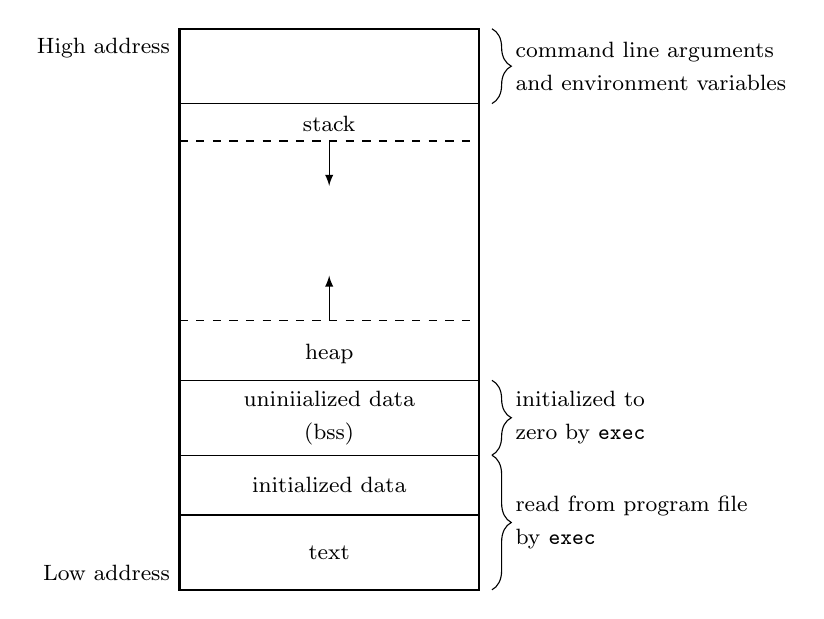
\begin{tikzpicture}[scale=0.95]
      % the box
      \draw [black, thick] (0,0) rectangle (4,7.5);
      \node [align=right, above left] at (0, 0) {\footnotesize Low address};
      \node [align=right, below left] at (0, 7.5) {\footnotesize High address};

      % high address before stack
      \uncover<2->{ \draw [black, thin] (0,6.5) -- (4,6.5);}
      % brace
      \uncover<2->{ \draw [decorate,decoration={brace,amplitude=7pt},xshift=5pt,yshift=0pt] (4,7.5) -- (4,6.5) node [black,align=left,midway,right, xshift=5pt] {\footnotesize command line arguments \\ \footnotesize and environment variables}; }

      % text
      \uncover<3->{ \draw [black, thin] (0,0) rectangle (4,1) node [black, align=center, midway] {\footnotesize text};}
      % initialized data
      \uncover<4->{ \draw [black, thin] (0,1) rectangle (4,1.8) node [black, align=center, midway] {\footnotesize initialized data};}
      % brace
      \uncover<4->{ \draw [decorate,decoration={brace,amplitude=7pt},xshift=5pt,yshift=0pt] (4,1.8) -- (4,0) node [black,align=left,midway,right, xshift=5pt] {\footnotesize read from program file \\ \footnotesize by \texttt{exec}};}
      % uninitialized data
      \uncover<5->{ \draw [black, thin] (0,1.8) rectangle (4,2.8) node [black, align=center, midway] {\footnotesize uniniialized data \\ \footnotesize (bss)};}
      % brace
      \uncover<5->{ \draw [decorate,decoration={brace,amplitude=7pt},xshift=5pt,yshift=0pt] (4,2.8) -- (4,1.8) node [black,align=left,midway,right, xshift=5pt] {\footnotesize initialized to \\ \footnotesize zero by \texttt{exec}};}

      % stack
      \uncover<6->{ \draw [dashed, thin] (0, 6) -- (4,6) node [black, align=center, midway, above] {\footnotesize stack};}
      % arrow down
      \uncover<6->{ \draw [arrows=-latex] (2,6) -- (2, 5.4);}

      % heap
      \uncover<7->{ \draw [dashed, thin] (0, 3.6) -- (4,3.6) node [black, align=center, midway, below, yshift=-5pt] {\footnotesize heap};}
      % arrow up
      \uncover<7->{ \draw [arrows=-latex] (2,3.6) -- (2, 4.2);}
    \end{tikzpicture}\\[1em]
    \caption{Typical Memory arrangement}
\label{fig:memory}
\end{figure}

\end{frame}

\begin{frame}[containsverbatim,t]
  \frametitle{Shared Libraries}
\texttt{size(1)} command reports the size (in bytes) of the text, data, and bss segments.

Mac does not support static linking of a library, but on Linux supports static linking.

Compare the size of a program before and after static linking.
\bigskip
{\footnotesize
\begin{columns}
  \begin{column}{0.4\linewidth}
    Dynamic linking
\begin{verbatim}
cc -o layout layout.c
file layout
ldd layout
size layout
objdump -d layout > obj_layout
wc -l obj_layout
\end{verbatim}
  \end{column}
  \begin{column}{0.45\linewidth}
    Static linking
\begin{verbatim}
cc -static -o layout_st layout.c
file layout_st
ldd layout_st
size layout_st
objdump -d layout_st > obj_layout_st
wc -l obj_layout_st
\end{verbatim}
  \end{column}
\end{columns}
}
\end{frame}


\begin{frame}[containsverbatim,t]
  \frametitle{Memory Allocation}

\begin{codedef}
#include <stdlib.h>
void *malloc(size_t size);
void *calloc(size_t nobj, size_t size);
void *realloc(void *ptr, size_t newsize);
// All three return: non-null pointer if OK, NULL on error

void free(void *ptr);
\end{codedef}
\begin{description}
\item[\texttt{malloc}] allocates a specified number of bytes of memory. The initial value of the memory is indeterminate
\item[\texttt{calloc}] allocates a specified number of bytes of memory and initializes them to 0 bits
\item[\texttt{realloc}] increases or decreases the size of a preivously allocated area
\item[\texttt{free}] deallocates the area. Do not \texttt{free} what is already freed
\end{description}

\end{frame}

\subsection{Misc.}

\begin{frame}[containsverbatim,t]
  \frametitle{\texttt{setjmp} and \texttt{longjmp} Functions}
In C, we can't \texttt{goto} a label that's in another function. Instead, we must use the \texttt{setjmp} and \texttt{longjmp} functions to perform this type of branching
\begin{codedef}
 #include <setjmp.h>
int setjmp(jmp_buf env);
// Returns: 0 if called directly, nonzero if returning from a call to longjmp
void longjmp(jmp_buf env, int val);
\end{codedef}
\begin{itemize}
\item call \texttt{setjmp} from the location that we want to return to.
  \begin{itemize}
  \item \texttt{jmp\_buf} data type is some form of array that is capable of holding all the information required to restore the status of the stack to the state when we call \texttt{longjmp}
  \end{itemize}
\item when we encounter an error, we call \texttt{longjmp} with two arguments
  \begin{itemize}
  \item \texttt{jmp\_buf env} used in \texttt{setjmp}
  \item \texttt{val} is nonzero value that becomes the return value from \texttt{setjmp}
  \end{itemize}
\end{itemize}
\end{frame}

\begin{comment}
\subsection{Last Words}

\begin{frame}
  \frametitle{Last Words}
  \begin{itemize}
  \item read chapter 8
  \end{itemize}
\end{frame}
\end{comment}
\end{document}
